\section{Framework measurements\label{sect:frame-measure}}

We describe in this section the results gathered with the extension approach described in the section \ref{sec:extension} and with the devices approach described in the section \ref{sec:external}.
For recall, the first approach is to implement the framework as a RTOS module used in the user space and that will compute internally the context switching time.
The second approach is to measure the context switching time using an external board, the PSLab.

In the same way as with the reference value, the results are divided by boards.
The measurements made with the RE-Mote boards are first given, then the one made with Z1 board.
The Contiki measurements are displayed side-by-side with the RIOT one for more clarity.

\subsection{Extension approach measurements}

\subsubsection{RE-Mote board measurements}
With Contiki, the framework outputs measurements with an average of 31.6162 $\mu$s.
With 0 $\mu$s as the minimum value and 457.7636 $\mu$s as the maximum value, the measurements have a large distribution.
We have a difference of 13.1112 $\mu$s between the measured context switching time and the real one measured with the oscilloscope.

With RIOT, the framework outputs a constant context switching time of 17 $\mu$s.
All 1000 measurements were equal to 17 $\mu$s.
Thus, the difference with the real context switching time is 4.374 $\mu$s.

Both measurements were above the real context switching time given by the reference value.
The table \ref{tab:extension-framework-remote} shows the measurement of Contiki and RIOT for the RE-Mote board.

\begin{table}[!ht]
  \centering
  \begin{tabular}{l|c|c}
                & Contiki  & RIOT \\ \hline
  Mean ($\mu$s) & 31.6162  & 17      \\
  Min  ($\mu$s) & 0        & 17      \\
  Max  ($\mu$s) & 457.7636 & 17     
  \end{tabular}
  \caption{extension approach measurements for Contiki and RIOT on the RE-Mote board}
  \label{tab:extension-framework-remote}
  \end{table}

\subsubsection{Z1 board measurements}
On the Class-1 Z1 board, the framework gave an average context switching time of 90.5761 $\mu$s with Contiki.
Once again, on Contiki, our values were largely distributed between 30.5175 $\mu$s and 976.5625 $\mu$s.
The average context switching time measured is 35.4991 $\mu$s above the real context switching time.

With RIOT, most of the values were equal to 40 $\mu$s with an average of 40.252 $\mu$s.
This put the measurements 12.553 $\mu$s above the real context switching time.

The table \ref{tab:extension-framework-z1} shows the measurement of Contiki and RIOT for the Z1 board.

\begin{table}[!ht]
  \centering
  \begin{tabular}{l|c|c}
                & Contiki  & RIOT \\ \hline
  Mean ($\mu$s) & 90.5761  & 40.252      \\
  Min  ($\mu$s) & 30.5175  & 40      \\
  Max  ($\mu$s) & 976.5625 & 41     
  \end{tabular}
  \caption{extension approach measurements for Contiki and RIOT on the Z1 board}
  \label{tab:extension-framework-z1}
  \end{table}

\subsection{Devices approach measurement}

\subsubsection{RE-Mote board measurements}
On the RE-Mote board, the devices approach outputs an average context switching time of 19.0329 $\mu$s on Contiki.
This measurement differs from the real context switching time by only 2.85$\%$.
They are 0.5279 $\mu$s above the reference measurements.
The majority of the values were around 14 $\mu$s but some of them were above 40 $\mu$s.
The figure \ref{fig:devices-framework-contiki-remote} show the distribution of the measurements made with Contiki.

\begin{figure}[!ht]
      \centering
      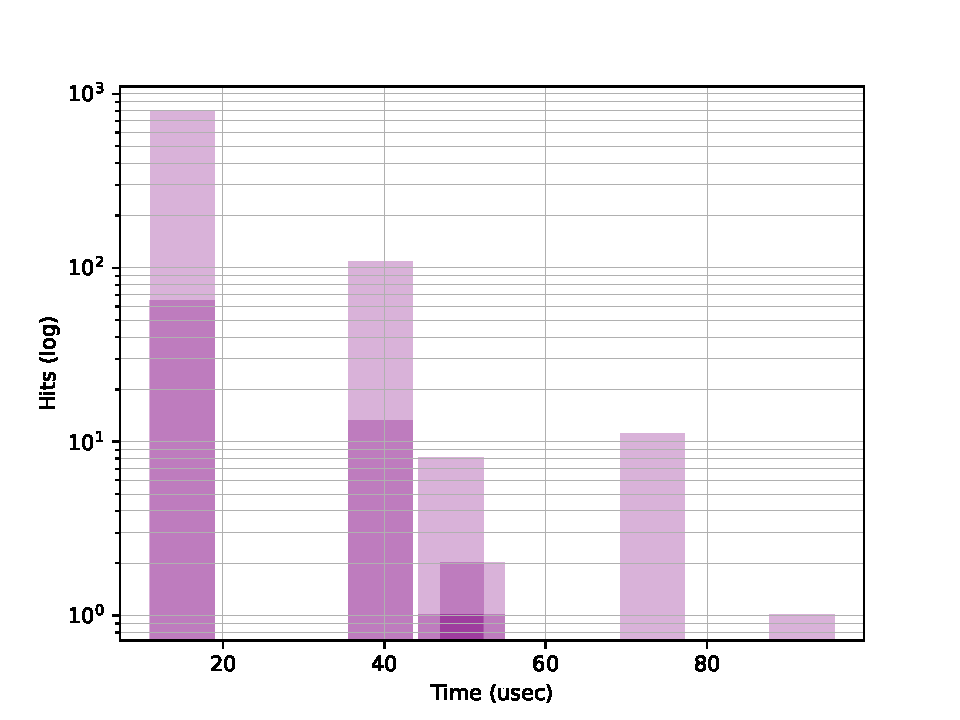
\includegraphics[scale=.7]{assets/devices-framework-contiki-remote.pdf}
      \caption{devices approach measurements distribution with Contiki on the RE-Mote board\label{fig:devices-framework-contiki-remote}}
\end{figure}

With RIOT, the average context switching was 12.9832 $\mu$s.
For RIOT, the measurements were either around 12.95 $\mu$s or around 13 $\mu$s.
The figure \ref{fig:devices-framework-riot-remote} shows this disparity.
The measured context switching time is above the real context switching time by 0.3572 $\mu$s.
This represents an offset of $2.82\%$ from the reference measurements.

\begin{figure}[!ht]
      \centering
      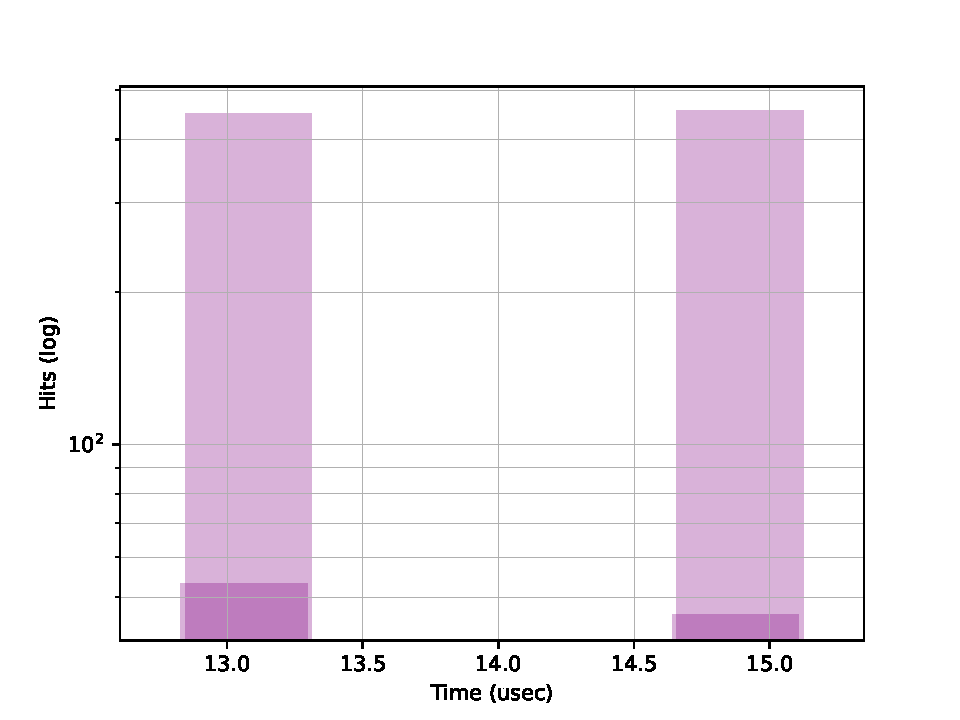
\includegraphics[scale=.7]{assets/devices-framework-riot-remote.pdf}
      \caption{devices approach measurements distribution with RIOT on the RE-Mote board\label{fig:devices-framework-riot-remote}}
\end{figure}

The table \ref{tab:devices-framework-remote} shows the measurement for Contiki and RIOT for the RE-Mote board.

\begin{table}[!ht]
  \centering
  \begin{tabular}{l|c|c}
                & Contiki  & RIOT \\ \hline
  Mean ($\mu$s) & 19.0329  & 12.9823 \\
  Min  ($\mu$s) & 14.9375  & 12.9375 \\
  Max  ($\mu$s) & 91.75    & 13.0156
  \end{tabular}
  \caption{devices framework measurements for Contiki and RIOT on the RE-Mote board}
  \label{tab:devices-framework-remote}
  \end{table}

\subsubsection{Z1 board measurements}
With the second approach, on the Z1 board, the framework found an average context switching time of 54.99 $\mu$s with Contiki.
The framework measurements were $0.15\%$ off from the real measurements by being 0.087 $\mu$s below them.
However, with Contiki the measured values are more scattered like shown in the figure \ref{fig:devices-framework-contiki-z1}.
The minimum measured context switching time is 32.5625 $\mu$s and the maximum one is 314.5 $\mu$s.

\begin{figure}[!ht]
      \centering
      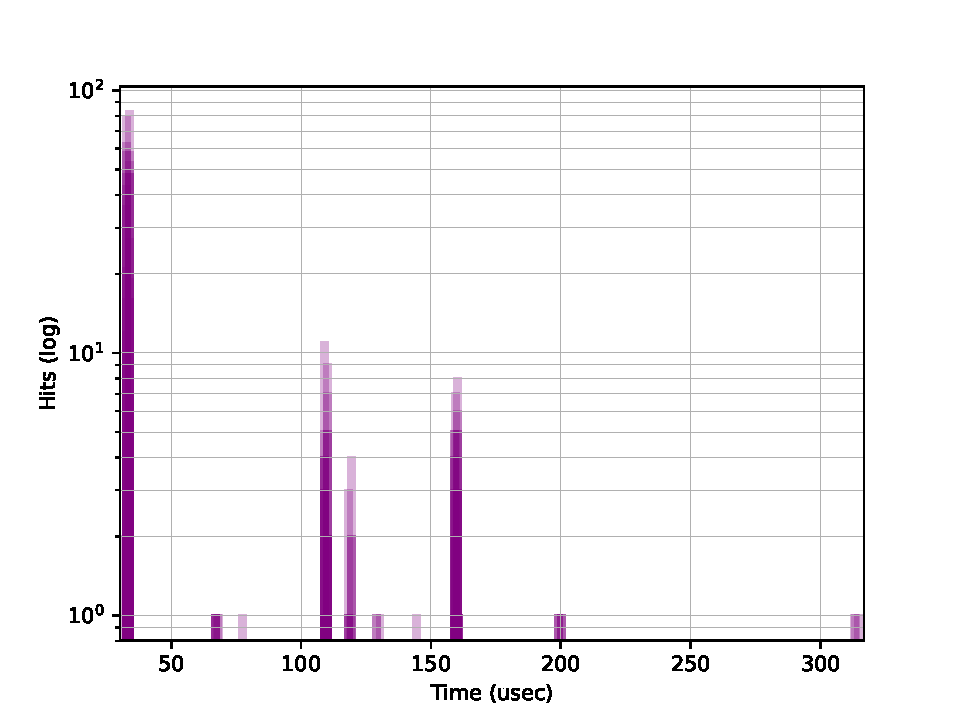
\includegraphics[scale=.7]{assets/devices-framework-contiki-z1.pdf}
      \caption{devices approach measurements distribution with Contiki on the Z1 board\label{fig:devices-framework-contiki-z1}}
\end{figure}

With RIOT, the framework outputted an average context switching time of 30.6971 $\mu$s.
The difference with the real context switching time is 2.9981 $\mu$s making the framework measurements more than $10\%$ above the reference measurements.
On the other hand, the framework measurements gave the same distribution as the one found with the oscilloscope in the section \ref{sec:ref-measurements} with the figure \ref{fig:reference-value-riot-z1}.
The measured measurements distribution is shown in the figure \ref{fig:devices-framework-riot-z1}.

\begin{figure}[!ht]
      \centering
      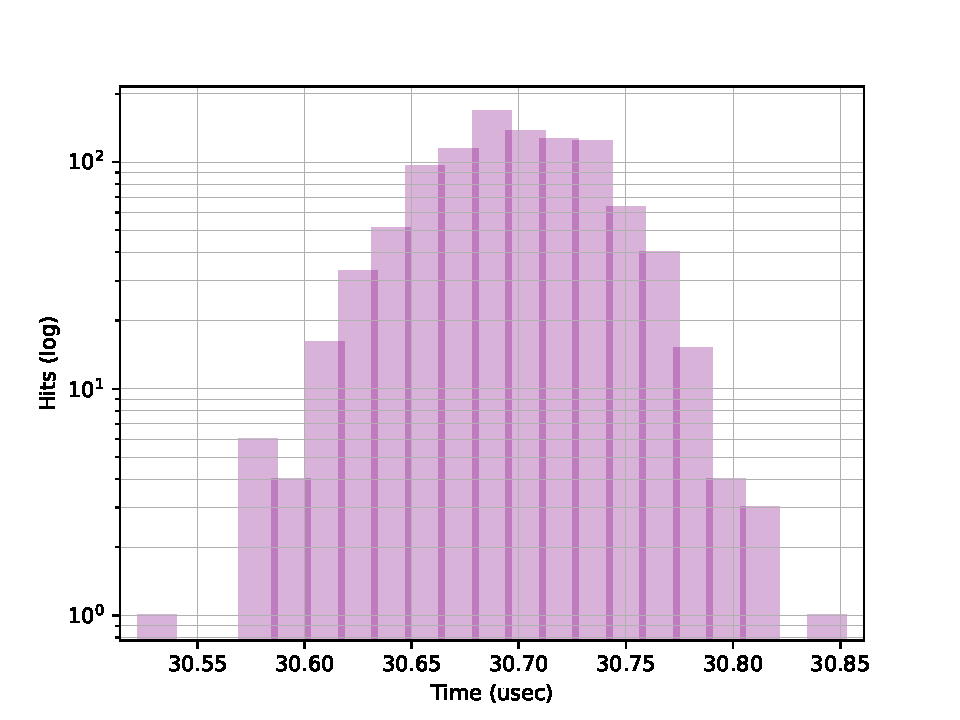
\includegraphics[scale=.7]{assets/devices-framework-riot-z1.pdf}
      \caption{devices approach measurements distribution with RIOT on the Z1 board\label{fig:devices-framework-riot-z1}}
\end{figure}

The table \ref{tab:devices-framework-z1} shows the measurement for both Contiki and RIOT on the Z1 board.

\begin{table}[!ht]
  \centering
  \begin{tabular}{l|c|c}
                & Contiki  & RIOT OS \\ \hline
  Mean ($\mu$s) & 54.99    & 30.6971 \\
  Min  ($\mu$s) & 32.5625  & 30.5312 \\
  Max  ($\mu$s) & 314.5    & 30.8437
  \end{tabular}
  \caption{devices framework measurements for Contiki and RIOT on the Z1 board}
  \label{tab:devices-framework-z1}
  \end{table}

\subsection{Summary}
To give more clarity to the results, the following tables give the average context switching time measured with the two approaches.
The table \ref{tab:framework-measurements-resume-remote} gives the measurements made on the RE-Mote board.
The table \ref{tab:framework-measurements-resume-z1} gives the measurements made on the Z1 board.
The difference between the measured context switching time and the real context switching time measured with the oscilloscope is written between parenthesis.

\begin{table}[!ht]
  \centering
  \begin{tabular}{l|c|c}
                      & Contiki           & RIOT             \\ \hline
  Extension approach ($\mu s$) & 31.6162 (13.1112) & 17 (4.374)       \\
  Devices approach ($\mu s$)   & 19.0329 (0.5279)  & 12.9832 (0.3572)
  \end{tabular}
  \caption{Framework measurements resume on the RE-Mote board}
  \label{tab:framework-measurements-resume-remote}
  \end{table}

\begin{table}[!ht]
  \centering
  \begin{tabular}{l|c|c}
                      & Contiki           & RIOT             \\ \hline
  Extension framework ($\mu s$) & 90.5761 (35.4991) & 40.252 (12.553)       \\
  Devices framework ($\mu s$)   & 54.99 (-0.087)  & 30.6971 (2.9981)
  \end{tabular}
  \caption{Framework measurements resume on the Z1 board}
  \label{tab:framework-measurements-resume-z1}
  \end{table}
